\documentclass[../main.tex]{subfiles}
\graphicspath{{\subfix{../images/}}}
\begin{document}
\textbf{ Quelques Images du Thème}
    \begin{figure}[bh]
        \centering
                \caption{In His LAB}
        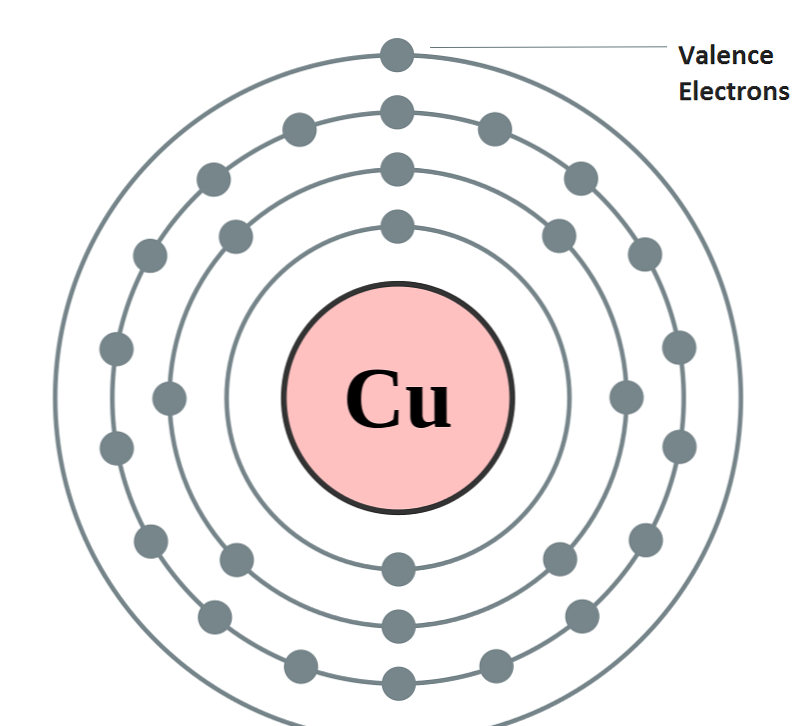
\includegraphics[width=6cm]{00-cu-difference-between-valency-and-valence-electrons_2} 
         \caption{00-cu-difference-between-valency-and-valence-electrons_2}
        \label{fig:img1}
            \end{figure}
    
    \begin{enumerate}
   \item First level item
   \item First level item
   \begin{enumerate}
     \item Second level item
     \item Second level item
     \begin{enumerate}
       \item Third level item
       \item Third level item
       \begin{enumerate}
         \item Fourth level item
         \item Fourth level item
       \end{enumerate}
     \end{enumerate}
   \end{enumerate}
 \end{enumerate}
    
    
\end{document}